\documentclass[tikz,border=2pt]{standalone}
\usepackage{amsmath,amssymb}
\usepackage{pgfplots}
\pgfplotsset{compat=1.18}

\begin{document}
% Survival functions: X1 ~ Exp(1), X2 ~ Exp(2) and their minimum. P(min > t) is the product
% of the two survival probabilities, e^{-t} e^{-2t} = e^{-3t}: again exponential, rate 1 + 2.
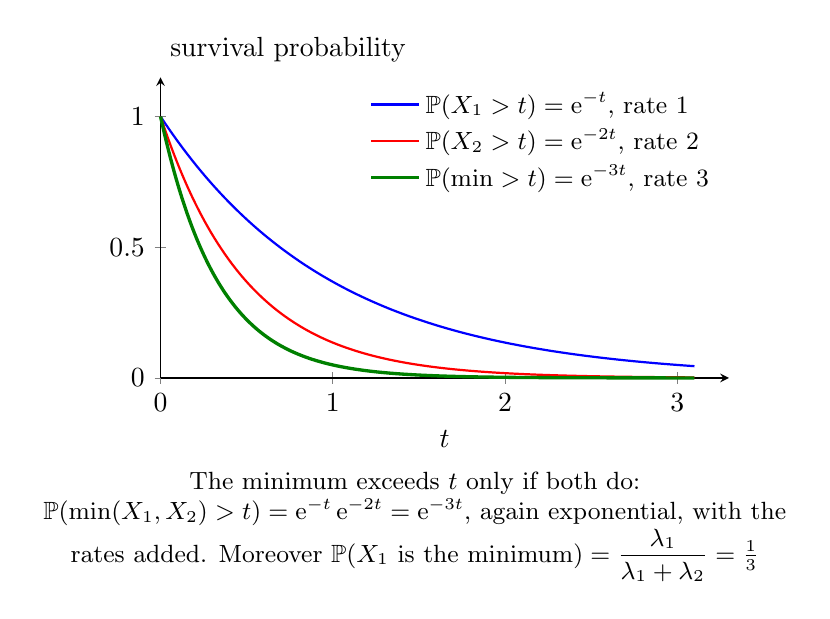
\begin{tikzpicture}
	\begin{axis}[
		axis lines=left, xmin=0, xmax=3.3, ymin=0, ymax=1.15,
		xtick={0,1,2,3}, ytick={0,0.5,1},
		xlabel={$t$}, ylabel={survival probability}, ylabel style={rotate=-90, anchor=south west, at={(axis description cs:0,1.02)}},
		samples=120, smooth, width=8.8cm, height=5.4cm, clip=false,
		legend style={draw=none, fill=none, font=\small, at={(0.99,0.99)}, anchor=north east}, legend cell align=left
		]
		\addplot[blue, thick, domain=0:3.1] {exp(-x)};
		\addlegendentry{$\mathbb{P}(X_1>t)=\mathrm{e}^{-t}$, rate $1$}
		\addplot[red, thick, domain=0:3.1] {exp(-2*x)};
		\addlegendentry{$\mathbb{P}(X_2>t)=\mathrm{e}^{-2t}$, rate $2$}
		\addplot[green!50!black, very thick, domain=0:3.1] {exp(-3*x)};
		\addlegendentry{$\mathbb{P}(\min>t)=\mathrm{e}^{-3t}$, rate $3$}
	\end{axis}
	\node[anchor=north, font=\small, align=flush center, text width=9.6cm] at ([yshift=-2pt]current axis.outer south) {The minimum exceeds $t$ only if both do: $\mathbb{P}(\min(X_1,X_2)>t)=\mathrm{e}^{-t}\,\mathrm{e}^{-2t}=\mathrm{e}^{-3t}$, again exponential, with the rates added. Moreover $\mathbb{P}(X_1\text{ is the minimum})=\dfrac{\lambda_1}{\lambda_1+\lambda_2}=\tfrac13$};
\end{tikzpicture}
\end{document}
